	\paragraph{QuizziPedia::Front-End::AppRun}
		
		\label{QuizziPedia::Front-End::AppRun}
		
		\begin{figure}[ht]
			\centering
			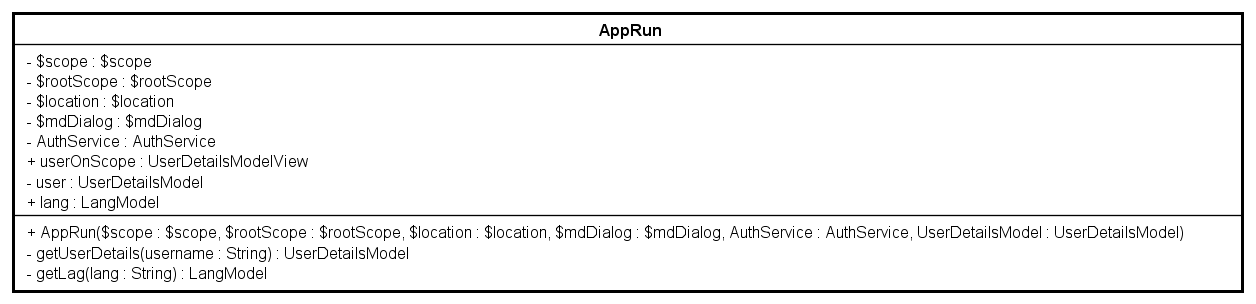
\includegraphics[scale=0.45,keepaspectratio]{UML/Classi/Front-End/QuizziPedia_Front-end_AppRun.png}
			\caption{QuizziPedia::Front-End::AppRun}
		\end{figure} \FloatBarrier
		
		\begin{itemize}

			\item \textbf{Descrizione}: classe che istanza l'applicazione;
			\item \textbf{Utilizzo}: viene utilizzata per indicare le dipendenze tra l'applicazione con i \textit{packages\ped{G}} esterni;

			\item \textbf{Attributi}: 
			\begin{itemize}
				\item \texttt{-} \texttt{ngRoute: ngRoute} \\
				Campo dati contenente un riferimento all'oggetto ngRoute creato da \textit{Angular\ped{G}};
				\item \texttt{-} \texttt{ngAnimate: ngAnimate} \\
				Campo dati contenente un riferimento all'oggetto ngAnimate creato da \textit{Angular\ped{G}};
				\item \texttt{-} \texttt{ngMaterial: ngMaterial} \\
				Campo dati contenente un riferimento all'oggetto ngMaterial creato dal \textit{package\ped{G}} \textit{Material Angular\ped{G}};
				\item \texttt{-} \texttt{ngMessages: ngMessages} \\
				Campo dati contenente un riferimento all'oggetto ngMessages creato da \textit{Angular\ped{G}};
				\item \texttt{-} \texttt{ngCookies: ngCookies} \\
				Campo dati contenente un riferimento all'oggetto ngCookies creato da \textit{Angular\ped{G}};
				\item \texttt{-} \texttt{ngFileUpload: ngFileUpload} \\
				Campo dati contenente un riferimento all'oggetto ngFileUpload creato dal \textit{package\ped{G}} \textit{ng-file-upload\ped{G}};
				\item \texttt{-} \texttt{angularCSS: angularCSS} \\
				Campo dati contenente un riferimento all'oggetto angularCSS creato dal \textit{package\ped{G}} \textit{AngularCSS\ped{G}};
				\item \texttt{-} \texttt{ui.bootstrap: ui.bootstrap} \\
				Campo dati contenente un riferimento all'oggetto ui.bootstrap creato dal \textit{package\ped{G}} \textit{AngularUI\ped{G}};
				\item \texttt{-} \texttt{ngDragDrop: ngDragDrop} \\
				Campo dati contenente un riferimento all'oggetto ngDragDrop creato dal \textit{package\ped{G}} \textit{Drag and Drop for AngularJS\ped{G}};
				\item \texttt{-} \texttt{angularNumberPicker: angularNumberPicker} \\
				Campo dati contenente un riferimento all'oggetto angularNumberPicker creato dal \textit{package\ped{G}} \textit{angular-number-picker\ped{G}};
				\item \texttt{-} \texttt{angles: angles} \\
				Campo dati contenente un riferimento all'oggetto angles creato dal \textit{package\ped{G}} \textit{Angles.js\ped{G}}.
			\end{itemize}
			\item \textbf{Metodi}: 
			\begin{itemize}
				\item \texttt{+} \texttt{InitialSetting(\$mdThemingProvider: \$mdThemingProvider): void} \\
				Metodo che imposta il tema dell'applicazione. \\
				\textbf{Parametri}:
				\begin{itemize}
					\item \texttt{\$mdThemingProvider: \$mdThemingProvider}\\ Parametro contenente un riferimento al servizio di \textit{Angular Material\ped{G}} che si occupa di configurare il tema dell'applicazione.
				\end{itemize}			
			\end{itemize}
		\end{itemize}
		